\documentclass[tikz,border=15pt]{standalone}
\usepackage{helvet}
\renewcommand{\familydefault}{\sfdefault}
\usepackage{tikz}
\usetikzlibrary{arrows.meta, positioning, fit, calc, shapes.geometric, decorations.pathreplacing, backgrounds}

\definecolor{emeraldpine}{HTML}{1A4D3E}
\definecolor{harvardcrimson}{HTML}{A51C30}
\definecolor{ethdarkblue}{HTML}{1F407A}
\definecolor{ethpetrol}{HTML}{007A87}
\definecolor{ethbronze}{HTML}{B87333}
\definecolor{ethpurple}{HTML}{5B4B8A}
\definecolor{ink}{HTML}{1A202C}
\definecolor{softink}{HTML}{4A5568}
\definecolor{paleink}{HTML}{A0AEC0}
\definecolor{cardbg}{HTML}{F8FAFC}
\definecolor{shadecolor}{HTML}{F4F6F9}

\begin{document}
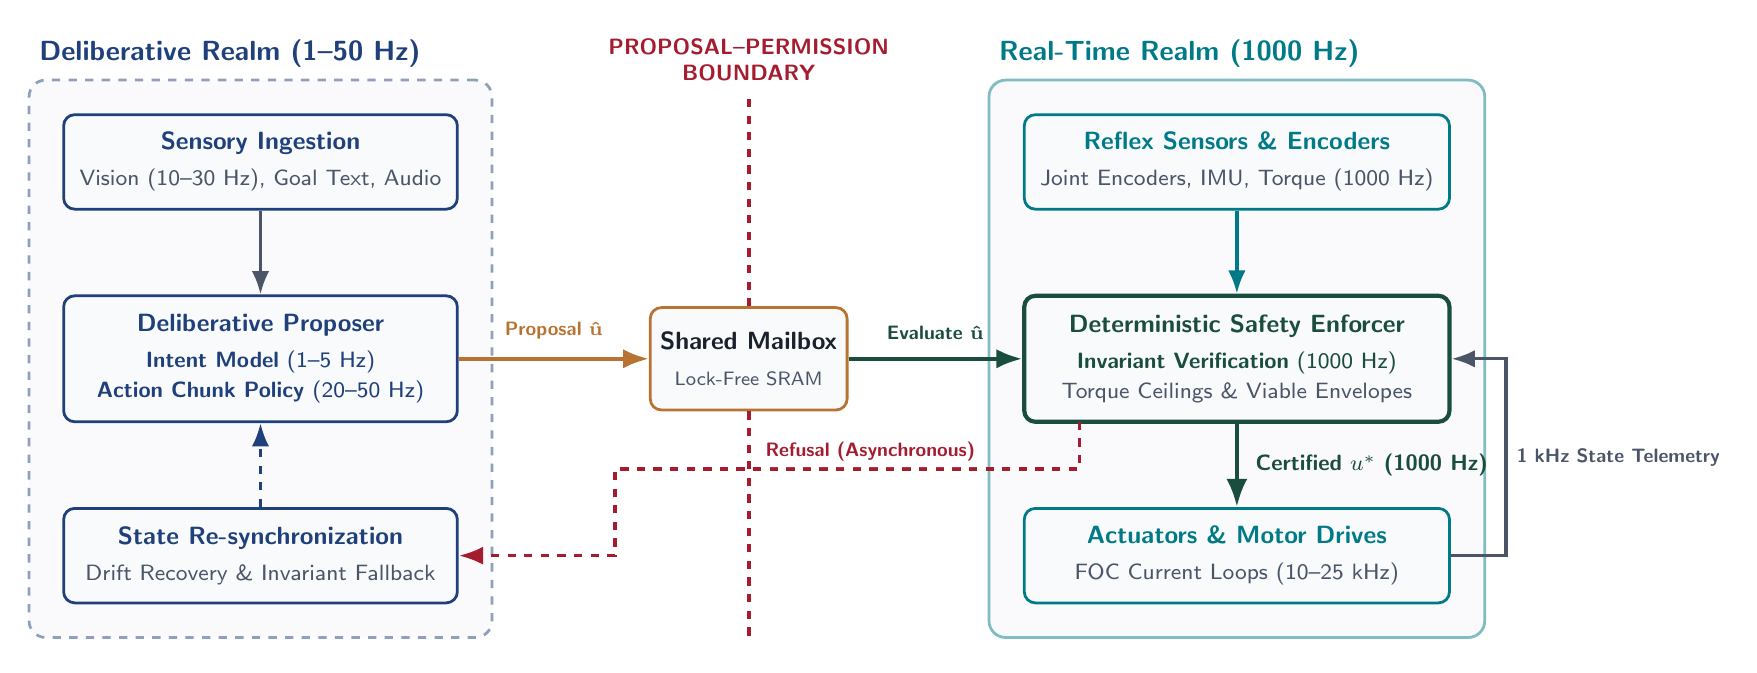
\begin{tikzpicture}[
    >=Latex,
    node distance=1.2cm and 2.5cm,
    box/.style={
        rectangle, 
        rounded corners=4pt, 
        draw, 
        fill=cardbg,
        minimum width=4.5cm, 
        minimum height=1.2cm,
        align=center,
        font=\sffamily\small\bfseries,
        line width=1pt
    },
    realm/.style={
        rectangle,
        rounded corners=6pt,
        draw,
        fill=shadecolor,
        inner sep=15pt,
        line width=1pt
    },
    arrow/.style={
        ->,
        line width=1.2pt,
        draw=softink
    },
    label/.style={
        font=\sffamily\footnotesize\bfseries
    }
]

% Left Column (Deliberative Realm)
\node[box, draw=ethdarkblue, text=ethdarkblue, minimum width=5.0cm] (sensory) at (0, 2.5) {
    Sensory Ingestion\\[2pt]
    {\footnotesize\normalfont\color{softink}Vision (10--30 Hz), Goal Text, Audio}
};

\node[box, draw=ethdarkblue, text=ethdarkblue, minimum width=5.0cm, minimum height=1.6cm] (policy) at (0, 0) {
    Deliberative Proposer\\[2pt]
    {\footnotesize\normalfont\color{ethdarkblue}\textbf{Intent Model} (1--5 Hz)}\\
    {\footnotesize\normalfont\color{ethdarkblue}\textbf{Action Chunk Policy} (20--50 Hz)}
};

\node[box, draw=ethdarkblue, text=ethdarkblue, minimum width=5.0cm] (resync) at (0, -2.5) {
    State Re-synchronization\\[2pt]
    {\footnotesize\normalfont\color{softink}Drift Recovery \& Invariant Fallback}
};

% Connect Left Side
\draw[arrow] (sensory) -- (policy);
\draw[arrow, dashed, draw=ethdarkblue] (resync) -- (policy);

% Center Mailbox Node on Proposal Boundary
\node[box, draw=ethbronze, text=ink, fill=cardbg, minimum width=2.5cm, minimum height=1.3cm] (mailbox) at (6.2, 0) {
    \textbf{Shared Mailbox}\\[2pt]
    {\scriptsize\normalfont\color{softink}Lock-Free SRAM}
};

% Right Column (Real-Time Realm)
\node[box, draw=ethpetrol, text=ethpetrol, minimum width=5.4cm] (reflex) at (12.4, 2.5) {
    Reflex Sensors \& Encoders\\[2pt]
    {\footnotesize\normalfont\color{softink}Joint Encoders, IMU, Torque (1000 Hz)}
};

\node[box, draw=emeraldpine, text=emeraldpine, minimum width=5.4cm, minimum height=1.6cm, line width=1.5pt] (safety) at (12.4, 0) {
    Deterministic Safety Enforcer\\[2pt]
    {\footnotesize\normalfont\color{emeraldpine}\textbf{Invariant Verification} (1000 Hz)}\\
    {\footnotesize\normalfont\color{softink}Torque Ceilings \& Viable Envelopes}
};

\node[box, draw=ethpetrol, text=ethpetrol, minimum width=5.4cm] (actuators) at (12.4, -2.5) {
    Actuators \& Motor Drives\\[2pt]
    {\footnotesize\normalfont\color{softink}FOC Current Loops (10--25 kHz)}
};

% Connect Right Side vertically
\draw[arrow, draw=ethpetrol] (reflex) -- (safety);
\draw[arrow, draw=emeraldpine, line width=1.6pt] (safety) -- node[right, font=\sffamily\footnotesize\bfseries, text=emeraldpine, inner sep=6pt] {Certified $u^*$ (1000 Hz)} (actuators);

% 1 kHz loop
\draw[arrow, draw=softink] (actuators.east) -- ++(0.7,0) |- node[pos=0.25, right, font=\sffamily\scriptsize\bfseries, text=softink] {1 kHz State Telemetry} (safety.east);

% Realms
\begin{scope}[on background layer]
    % Left Realm Background
    \node[realm, draw=ethdarkblue!50, fill=shadecolor!50, dashed, fit=(sensory) (policy) (resync), inner sep=12pt] (leftrealm) {};
    \node[anchor=south west, text=ethdarkblue, font=\sffamily\bfseries, inner sep=4pt] at (leftrealm.north west) {Deliberative Realm (1--50 Hz)};
    
    % Right Realm Background
    \node[realm, draw=ethpetrol!50, fill=shadecolor!50, fit=(reflex) (safety) (actuators), inner sep=12pt] (rightrealm) {};
    \node[anchor=south west, text=ethpetrol, font=\sffamily\bfseries, inner sep=4pt] at (rightrealm.north west) {Real-Time Realm (1000 Hz)};
\end{scope}

% Boundary Line & Header
\node[font=\sffamily\footnotesize\bfseries, text=harvardcrimson, align=center, fill=white, rounded corners=2pt, inner sep=4pt] at (6.2, 3.8) {PROPOSAL--PERMISSION\\BOUNDARY};

\draw[line width=1.5pt, draw=harvardcrimson, dashed] 
    (6.2, 3.3) -- (mailbox.north)
    (mailbox.south) -- (6.2, -3.6);

% Cross-Boundary Signals
% Proposal \hat{u} into Mailbox
\draw[arrow, draw=ethbronze, line width=1.4pt] (policy.east) -- node[above=3pt, font=\sffamily\scriptsize\bfseries, text=ethbronze] {Proposal $\mathbf{\hat{u}}$} (mailbox.west);

% Read proposal from Mailbox to Safety Enforcer
\draw[arrow, draw=emeraldpine, line width=1.4pt] (mailbox.east) -- node[above=3pt, font=\sffamily\scriptsize\bfseries, text=emeraldpine] {Evaluate $\mathbf{\hat{u}}$} (safety.west);

% Refusal from Safety Enforcer directly to Resync
\draw[arrow, draw=harvardcrimson, line width=1.3pt, dashed] 
    (10.4, -0.8) -- (10.4, -1.4) -- node[pos=0.45, above, font=\sffamily\scriptsize\bfseries, text=harvardcrimson, fill=white, inner sep=2pt, rounded corners=2pt] {Refusal (Asynchronous)} (4.5, -1.4) |- (resync.east);

\end{tikzpicture}
\end{document}
